\documentclass[12pt]{article}


\usepackage[english]{babel}
\usepackage[utf8]{inputenc}
\usepackage{amsmath,amssymb}
\usepackage{listings} % untuk kode python
\usepackage{xcolor}

\definecolor{codegreen}{rgb}{0,0.6,0}
\definecolor{codegray}{rgb}{0.5,0.5,0.5}
\definecolor{codepurple}{rgb}{0.58,0,0.82}
\definecolor{backcolour}{rgb}{0.95,0.95,0.92}

\lstdefinestyle{mystyle}{
    backgroundcolor=\color{backcolour},   
    commentstyle=\color{codegreen},
    keywordstyle=\color{magenta},
    numberstyle=\tiny\color{codegray},
    stringstyle=\color{codepurple},
    basicstyle=\ttfamily\footnotesize,
    breakatwhitespace=false,         
    breaklines=true,                 
    captionpos=b,                    
    keepspaces=true,                 
    numbers=left,                    
    numbersep=5pt,                  
    showspaces=false,                
    showstringspaces=false,
    showtabs=false,                  
    tabsize=2
}

\lstset{style=mystyle}
%\usepackage{parskip}
\usepackage{graphicx}

% Margins
\usepackage[top=2.5cm, left=3cm, right=3cm, bottom=4.0cm]{geometry}
\usepackage{hyperref}
\usepackage{natbib}
\setlength\bibsep{1em}
\setlength\bibhang{1.5em}
\renewcommand\bibfont{\singlespace}
\bibliographystyle{dcu}
% Colour table cells
%\usepackage[table]{xcolor}

% Get larger line spacing in table
\newcommand{\tablespace}{\\[1.25mm]}
\newcommand\Tstrut{\rule{0pt}{2.6ex}}         % = `top' strut
\newcommand\tstrut{\rule{0pt}{2.0ex}}         % = `top' strut
\newcommand\Bstrut{\rule[-0.9ex]{0pt}{0pt}}   % = `bottom' strut

%%%%%%%%%%%%%%%%%
%     Title     %
%%%%%%%%%%%%%%%%%
\title{Exercise 1 - Linear Regression}
\author{Azka NA}
\date{\today}

\begin{document}
\maketitle

%%%%%%%%%%%%%%%%%
%   Problem 1   %
%%%%%%%%%%%%%%%%%
\section{Introduction}
This is the guide for Andrew Ng's Machine Learning course programming assignment done in Python, adapted from the original guide written for Octave or MATLAB.

In this exercise, you will implement linear regression and get to see it work on data. Before starting on this programming exercise, we strongly recommend watching the video lectures and completing the review questions for the associated topics

For Programming Exercise 1: Linear Regression, you will need to download the following files:

\texttt{exercise1.ipynb} - Jupyter notebook containing the script through the exercise

\texttt{ex1data1.txt} - Dataset for linear regression with one variable

\texttt{ex1data2.txt} - Dataset for linear regression with multiple variables

\section{Linear regression with one variable}

In this part of this exercise, you will implement linear regression with one variable to predict profits for a food truck. Suppose you are the CEO of a restaurant franchise and are considering different cities for opening a new outlet. The chain already has trucks in various cities and you have data for profits and populations from the cities.

You would like to use this data to help you select which city to expand to next.

The file \texttt{ex1data1.txt} contains the dataset for our linear regression problem. The first column is the population of a city and the second column is the profit of a food truck in that city. A negative value for profit indicates a loss.

\subsection{Plotting the Data}
Before starting on any task, it is often useful to understand the data by visualizing it. For this dataset, you can use a scatter plot to visualize the data, since it has only two properties to plot (profit and population). (Many other problems that you will encounter in real life are multi-dimensional and can’t be plotted on a 2-d plot.)

In \texttt{exercise1.ipynb}, the dataset is loaded from the data file into variables $X$ and $y$:
\begin{lstlisting}[language=Python]
    import pandas as pd 

    dataset = pd.read_csv('ex1data1.txt', header=None, names=['population', 'profit'])
    X = dataset.iloc[:,0]
    y = dataset.iloc[:,1]
    m = len(y)
\end{lstlisting}

Next, we create a scatter plot of the data with the following code. The end result should look like Figure~\ref{fig:scatter1}.

\begin{lstlisting}[language=Python]
    import matplotlib.pyplot as plt

    plt.scatter(X, y, marker='x', c='red')
    plt.ylabel('Profit in $10,000s')
    plt.xlabel('Population of City in 10,000s')
    plt.show()
\end{lstlisting}

\begin{figure}[h!]
  \centering
  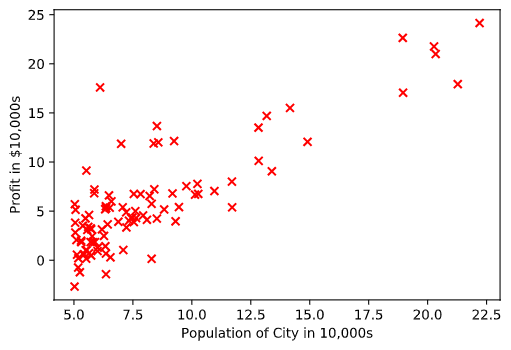
\includegraphics[scale=0.6]{scatter1.png}
  \caption{Scatter plot of training data}
  \label{fig:scatter1}
\end{figure}

\subsection{Gradient Descent}
In this part, you will fit the linear regression parameters $\theta$ to our dataset using gradient descent.
\subsubsection{Adding the intercept term}
In the following lines, we add another dimension to our data to accommodate the $\theta_0$ intercept term. We also initialize the initial parameters to 0 and the learning rate \texttt{alpha} to 0.01.
\begin{lstlisting}[language=Python]
    import numpy as np
    
    X = X[:,np.newaxis]
    y = y[:,np.newaxis]
    theta = np.zeros([2,1])

    alpha = 0.01
    iterations = 1500
    ones = np.ones((m,1))
    X = np.hstack((ones, X)) # adding the intercept term
\end{lstlisting}

"Note on \texttt{np.newaxis}: When you read data into $X$, y you will observe that $X$, $y$ are rank 1 arrays. rank 1 array will have a shape of (m, ) where as rank 2 arrays will have a shape of (m,1). When operating on arrays its good to convert rank 1 arrays to rank-2 arrays because rank-1 arrays often give unexpected results. To convert rank 1 to rank 2 array we use \texttt{someArray[:,np.newaxis]}." \citep{srikar2018}

The \texttt{X = X[:, np.newaxis]} line will change the $X$ matrix into:

\begin{align}
  \mathbf x = \begin{bmatrix} x^{(i)} \\ .. \\ x^{(m)}  
  \end{bmatrix} \\
  \mathbf x = \begin{bmatrix} x^1 \\ x^2 \\ x^3 \\ .. \\ x^m\end{bmatrix}
\end{align}

After adding the intercept term, we will get $X$ matrix which has column 1 as the intercept $(\theta_0)$ and column 2 as the feature value.

\begin{align}
  \mathbf x = \begin{bmatrix} 1 & x^1 \\ 1 & x^2 \\ 1 & x^3 \\ .. & .. \\ 1 & x^m\end{bmatrix} \\
\end{align}

\subsubsection{Computing the cost $J(\theta)$}
As you perform gradient descent to learn minimize the cost function $J(\theta)$, it is helpful to monitor the convergence by computing the cost. In this section, you will implement a function to calculate $J(\theta)$ so you can check the convergence of your gradient descent implementation.
The next task is to make a function that computes $J(\theta)$. As you are doing this, remember that the variables $X$ and $y$ are not scalar values, but matrices whose rows represent the examples from the training set.
The \texttt{computeCost} function uses $\theta$ initialized to zeros and is based on the following simplified equation:
\begin{align}
    h_\theta(x) & = \theta_0 + \theta_1x  \\
    h_\theta(x) & = \theta_1x  \\
    \theta_0 & = 0 \\
    J(\theta_1) & = \frac{1}{2m}\sum_{i=1}^m{(h_\theta(x^{(i)})-y^{(i)})^2}
\end{align}

The code for \texttt{computeCost} function is:

\begin{lstlisting}[language=Python]
def computeCost(X, y, theta):
    '''check page 10 of "2 Linear regression with one variable"
    '''
    m = len(y)
    #err = X.dot(theta) - y (sama aja)
    err = np.dot(X, theta) - y
    return np.sum(np.power(err, 2)) / (2*m)
\end{lstlisting}

You should expect to see a cost of \texttt{32.07}

\subsubsection{Gradient descent}
Next, you will implement gradient descent using the \texttt{gradientDescent} function. The value of $\theta$ is updated within each iteration. Keep in mind that the cost $J(\theta)$ is parameterized by the vector $\theta$, not $X$ and $y$. That is, we minimize the value of $J(\theta)$ by changing the values of the vector $\theta$, not by changing $X$ or $y$. Refer to the equations in this handout and to the video lectures if you are uncertain.

A good way to verify that gradient descent is working correctly is to look at the value of $J(\theta)$ and check that it is decreasing with each step. The code for \texttt{gradientDescent} calls \texttt{computeCost} on every iteration and prints the cost. Assuming you have implemented gradient descent and \texttt{computeCost} correctly, your value of $J(\theta)$ should never increase, and should converge to a steady value by the end of the algorithm.

The code for \texttt{gradientDescent} is based on the following equation:

\begin{align}
    J(\theta_0, \theta_1) = \frac{1}{2m}\sum_{i=1}^m{(\hat{y_i}-y_i)^2} = \frac{1}{2m}\sum_{i=1}^m{(h_\theta(x^{(i)})-y^{(i)})^2}
\end{align}

\begin{align}
  \theta_0 & := \theta_9 - \alpha\frac{1}{m}\sum_{i=1}^m{(h_\theta(x^{(i)})-y^{(i)})}\\
  \theta_1 & := \theta_1 - \alpha\frac{1}{m}\sum_{i=1}^m{(h_\theta(x^{(i)})-y^{(i)})}\cdot x^{(i)}
\end{align}

The code for \texttt{gradientDescent} function is:

\begin{lstlisting}[language=Python]
def gradientDescent(X, y, theta, alpha, iterations):
    ''' check "2 Linear regression with one variable"
    page 36
    '''
    m = len(y)
    J_val = []
    for i in range(iterations):
        J = np.dot(X, theta) - y
        error = np.dot(X.T, J)
        descent = alpha*1/m*error
        theta -= descent
        J_val.append(computeCost(X, y, theta))
    return theta, J_val
\end{lstlisting}

Using the provided dataset, the expected \texttt{theta} value is \texttt{-3.63029144} and \texttt{1.16636235}.

The \texttt{gradientDescent} function also records the history of $J(\theta)$ for each iteration. We can check whether our iteration is converging, i.e. the $J(\theta)$ is decreasing after each iteration. The result would be something like Figure~\ref{fig:cost}.

\begin{lstlisting}[language=Python]
    theta1, J_values = gradientDescent(X, y, theta, alpha, iterations)
    plt.plot(np.arange(1,iterations+1), J_values)
    plt.show()
\end{lstlisting}

\begin{figure}[h!]
  \centering
  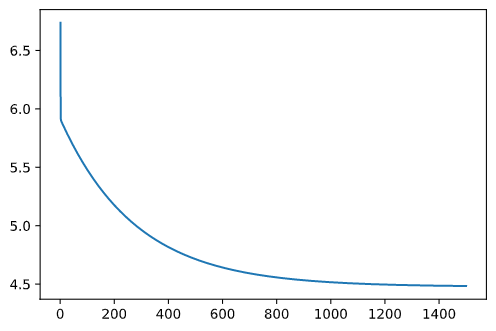
\includegraphics[scale=0.6]{cost.png}
  \caption{$J(\theta)$ for each iteration}
  \label{fig:cost}
\end{figure}

Your final values for $\theta$ will also be used to make predictions on profits in areas of 35,000 and 70,000 people. Using the $\theta$ calculated by \texttt{gradientDescent} earlier, the profit is:

\begin{lstlisting}[language=Python]
population = [3.5, 7] # 35000 and 70000 people
for pop in population:
    print(f'Expected profit in a city with {int(pop*10000)} people is ${int(np.dot([1,pop], theta1)[0]*10000)}')
\end{lstlisting}

\subsubsection{Plot with the best fit line}
We can draw the plot of the training data and the best fit line as shown in Figure~\ref{fig:bestfit}

\begin{figure}[h!]
  \centering
  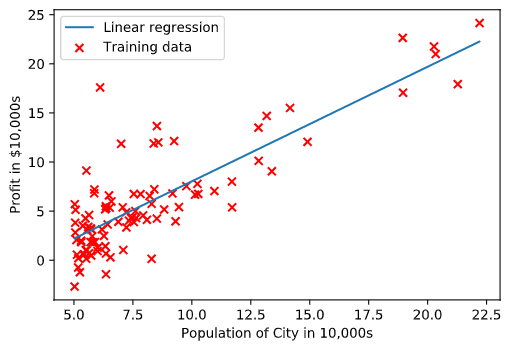
\includegraphics[scale=0.6]{bestfit.png}
  \caption{Best fit line for the training data}
  \label{fig:bestfit}
\end{figure}

\section{Linear regression with multiple variables}

In this part, you will implement linear regression with multiple variables to predict the prices of houses. Suppose you are selling your house and you want to know what a good market price would be. One way to do this is to first collect information on recent houses sold and make a model of housing prices.

The file \texttt{ex1data2.txt} contains a training set of housing prices in Portland, Oregon. The first column is the size of the house (in square feet), the second column is the number of bedrooms, and the third column is the price of the house.

\subsection{Feature Normalization}
First, load the dataset and look at the values. Note that the house sizes are about 1000 times the number of bedrooms. When features differ by orders of magnitude, first performing feature scaling can make gradient descent converge much more quickly.

\begin{lstlisting}[language = Python]
    dataset2 = pd.read_csv('ex1data2.txt', header=None, names=['size', 'bedrooms', 'price'])
    print(dataset2.head())
\end{lstlisting}

\begin{table}[h!]
  \centering
  \begin{tabular}{ r r r r } 
     & size & bedrooms & price \\
    \hline
    0 & 2104 & 3 & 399900 \\
    1 & 1600 & 3 & 329900 \\
    2 & 2400 & 3 & 369000 \\
    3 & 1416 & 2 & 232000 \\
    4 & 3000 & 4 & 539900 \\
    \hline
  \end{tabular}
\end{table}

Your task here is to:
\begin{itemize}
  \item Subtract the mean value of each feature from the dataset.
  \item After subtracting the mean, additionally scale (divide) the feature values by their respective "standard deviations."
\end{itemize}

The standard deviation is a way of measuring how much variation there is in the range of values of a particular feature (most data points will lie within $\pm$ 2 standard deviations of the mean); this is an alternative to taking the range of values (max-min).

\begin{lstlisting}[language=Python]
    X = dataset2.iloc[:,0:2] 
    y = dataset2.iloc[:,2]
    m = len(y)
    X_scaled = (X - np.mean(X))/np.std(X)

    ones = np.ones((m2,1))
    X_scaled = np.hstack((ones, X_scaled))
    alpha = 0.01
    iterations = 400
    theta = np.zeros((3,1)) # there are now 3 parameters
    y = y[:,np.newaxis]
\end{lstlisting}

\subsection{Gradient Descent}
Using the same \texttt{computeCost} function, we can get the cost of \texttt{65591548106.45744}.
\begin{lstlisting}
    J = computeCost(X_scaled, y, theta)
\end{lstlisting}

Then, using the same \texttt{gradientDescent} function, we can get the $\theta$ value of \texttt{334302}, \texttt{99411}, and \texttt{3267}.
\begin{lstlisting}[language=Python]
    theta1, J_values = gradientDescent(X_scaled, y, theta, alpha, iterations)
    print(theta1)
\end{lstlisting}

Using the computed value, \texttt{theta1}, we can compute the cost of the function, which was \texttt{2105448288}, far lower than the previous cost when the $\theta$ was 0, 0, and 0.

\begin{lstlisting}[language=Python]
  J = computeCostMulti(X_scaled, y, theta1)
\end{lstlisting}


\bibliography{mybib}

\end{document}
